\documentclass[main.tex]{subfiles}
\begin{document}

\section{ Частотные критерии устойчивости Михайлова и Найквиста }
5 марта 2021 г. \\

Темы важные, непростые.
Возможно, даже центральные! \\

Устойчивость -- основное свойство системы.
Как правило, все системы должны быть устойчивы.
Истребитель, в отличие от гражданского самолёта, в свободном полёте неустойчив, НО с помощью обратной связи мы вновь делаем его устойчивым!

\textbf{Напоминание:} для устойчивости линейной динамической системы достаточно выполнения условия
$$ \boxed{Re \lambda_i < 0} $$
где $ \lambda_i : \alpha(\lambda_i) = 0 $

Проверять корни характеристического полинома -- занятие неблагодарное.
Есть необходимое условие Стодола, а также н. и д. условие Гурвица.
Их дополняет критерий Льенара-Шипара.

\subsubsection{Частотные критерии. Введение}

На прошлом занятии мы разобрали, что такое частотные характеристики.
Зачем они нужны, если есть алгебраические?
Когда порядок системы большой (10, 100, ...), задача вычисления большого числа определителей также неблагодарная.
А на базе некоторых характеристик, которые мы будем называть \emph{годографами}, можно определить устойчивость проще.
Причём будет достаточно найти годографы лишь приближённо.
Знак определителя не найти с помощью приближённых вычислений!

\subsection{Критерий Михайлова}
1938 год.

Частотные характериристики основаны на \textbf{принципе аргумента} из теории функции комплексной переменной: приращение аргумента функции при обходе области
$$ \Delta \arg f(z) = 2 \pi (N - P) $$
здесь $N$ -- число нулей и $ P $ -- число полюсов внутри области.

Докажем в одном частном случае -- когда функция $f(z)$ -- полином, а $p$ пробегает по мнимой оси (нам этого достаточно).

$$ \alpha(p) = a_0 p^n + ... + a_n \overset{\text{th.  Безу}}= a_0 \prod_i (p - p_i), \thickspace \alpha(p_i) = 0 $$
где $ \alpha(p) $ -- характеристический полином, знаменатель некоторой передаточной функции $ H(p) = \frac{\beta(p)}{\alpha(p)} $.

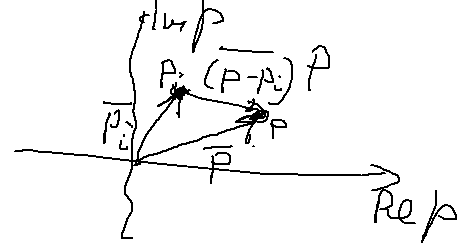
\includegraphics[width=.4\linewidth]{lec6/01_polynome_roots}

Пусть $p = j \omega $ (хотим располагаться на мнимой оси).
Пусть также для определённости $ a_0 > 0 $, т. е. $ \arg a_0 = 0 $.

Аргумент произведения есть сумма аргументов.
Аргумент $ a_0 $ равен нулю, если это положительное вещественное число.
$$ \arg \alpha(j \omega) = \sum_{i=1}^{n} \arg (j \omega - p_i) $$
Найдём приращение аргумента при перемещении точки от $ - \infty $ до $ + \infty $ по комплексной оси
$$ \Delta \arg \alpha(j \omega) |_{-\infty}^\infty = \sum_i \Delta \arg (j \omega - p_i) |_{-\infty}^\infty $$

Изобразим корни уравнения на комплексной плоскости:

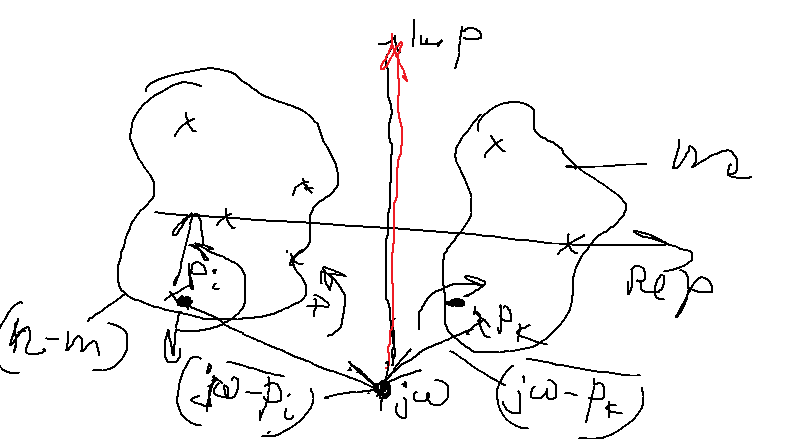
\includegraphics[width=.6\linewidth]{lec6/02_roots_jw}

Хотим посмотреть на приращение аргумента от каждого слагаемого $ p - p_i $ (и затем эти приращения просуммировать).
Пусть в правой полуплоскости $ m $ корней $ \Rightarrow $ в левой $ n - m $ (общий порядок $n$).

Условимся считать за положительное направление поворот против часовой стрелки.
От каждого вектора из левой полуплоскости приращение угла поворота при проходе $ \omega $ от $ - \infty $ до $ + \infty $ есть $ \pi $, от каждого правого -- $ \pi $. Тогда

$$ \Delta \arg \alpha(j \omega) |_{-\infty}^\infty = \pi (n - m) - \pi \cdot m = \pi (n - 2 m)  $$
Принцип аргумента в нашем частном случае доказан. \\

Нарисуем один из возможных годографов, то есть кривую $ \alpha(j \omega) |_{-\infty}^\infty $ в осях $ Re(\alpha(j \omega)), Im(\alpha(j \omega)) $.

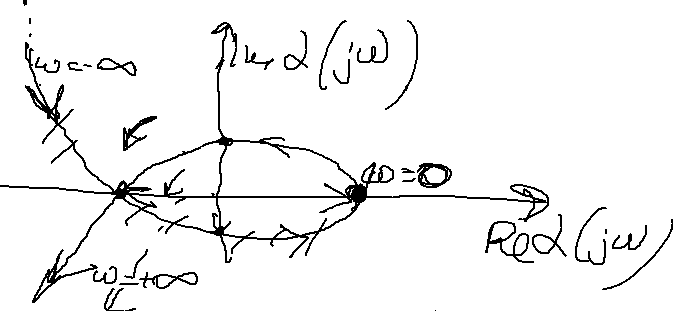
\includegraphics[width=.5\linewidth]{lec6/03_mikhailov_godograph}

Геометрическое место точек, образованное значениями полинома $ \alpha(j \omega) $ (точнее, её половину), называют \emph{кривой Михайлова}.

Пример.

\begin{align*}
    & \alpha(p) = p^2 + p + 1 \\
    & \alpha(j \omega) = 1 - \omega^2 + j \omega \\
    & \text{обозначим } X(\omega) = 1 - \omega^2, \thickspace Y(\omega) = \omega \\
    & \alpha(j \omega) = X(\omega) + j Y(\omega) \\
    & X(\omega) = X(-\omega) \Rightarrow \text{ годограф симметричен относительно вещественной оси} \\
    & Y(\omega) = Y(- \omega) \Rightarrow Y(\omega = 0) = 0 \\
\end{align*}

Приращение аргумента при движении по годографу от $ \omega = - \infty $до $ \omega = \infty $ есть$ 3 \pi $.
Поскольку кривая симметрична, можно рассматривать только его половину $ \alpha(j \omega) |_0^\infty $

На <<половинной>> кривой для нашего примера приращение аргумента $ 3\frac{\pi}{2} $, а в общем случае

\begin{equation}\label{eq:mikhailov}
	\boxed{ \Delta \arg \alpha (j \omega) |_0^\infty = \frac{\pi}{2} (n - 2m) }
\end{equation}

Для устойчивости необходимо и достаточно, чтобы $ m = 0 $ (нет правых, неустойчивых корней):
\begin{equation}\label{eq:mikh1}
\boxed{ \Delta \arg \alpha(j \omega) |_0^\infty = \frac{\pi}{2} n }
\end{equation}
Для асимптотической устойчивости также нужно, чтобы не было корней на мнимой оси:
\begin{equation}\label{eq:mikh2}
	\boxed{ \alpha(j \omega) \ne 0 }
\end{equation}
(т. о. годограф не должен проходить через начало координат). Пример хорошего годографа:

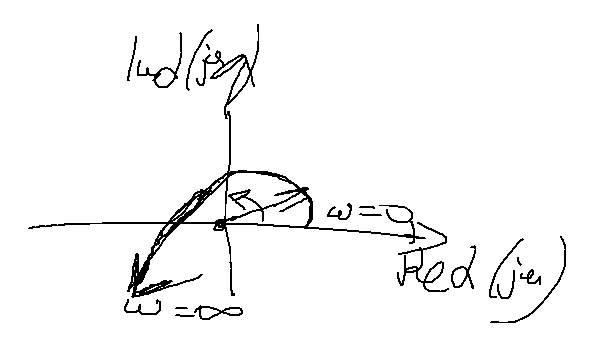
\includegraphics[width=.5\linewidth]{lec6/04_mikhailov_polyn_godograph}

Формулы \eqref{eq:mikh1} и \eqref{eq:mikh2} вместе и есть критерий Михайлова.

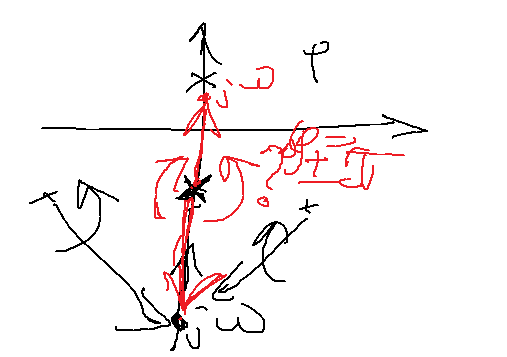
\includegraphics[width=.5\linewidth]{lec6/05_mikhailov_imaginary_roots}

Пояснение к формуле \eqref{eq:mikh2}:
если корень на мнимой оси, то приращение аргумента при его обходе -- $\pi$, но мы не знаем, с каким знаком.
То есть неопределённость: $ \Delta \arg j \omega = ? $

Это как деление на ноль -- если определим как предел, будет непонятно, какой знак: $ \frac{1}{0} = \lim\limits_{\varepsilon \to 0} \frac{1}{\varepsilon} = \pm \infty \Rightarrow $ неопределённость, не можем так определить. \\

\textbf{Замечания:}

\begin{enumerate}[noitemsep]
	\item Для устойчивой системы кривая Михайлова имеет вид спирали, которая стартует на вещественной оси, всё время монотонно раскручивается в одном направлении и заканчивается в квадранте $ n $ (т. е. $ \Delta \phi = n\frac{\pi}{2} $), $n$ -- порядок полинома $\alpha$.

    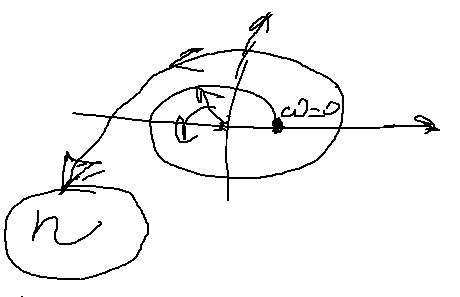
\includegraphics[width=.4\linewidth]{lec6/07_mikh_revolutions}

    Пример:

    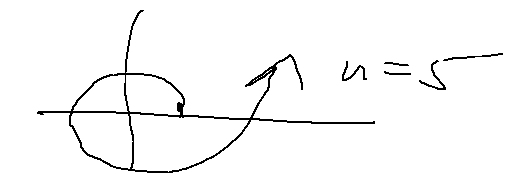
\includegraphics[width=.4\linewidth]{lec6/09_mikh_example1}

    Следующий годограф невозможен, если система устойчива:

    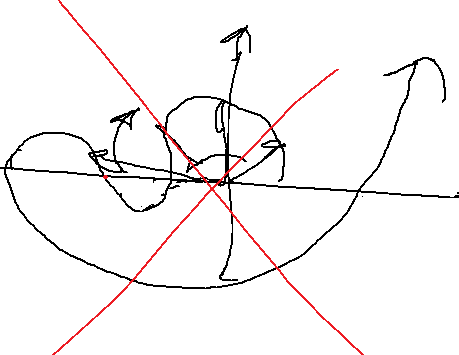
\includegraphics[width=.4\linewidth]{lec6/08_mikh_wrong_revolutions}

	Почему спираль монотонно раскручивается?
	Изменение аргумента от всякого корня с $ Re < 0 $ есть монотонная функция, и сумма их тоже.

    Смотрите, как замечательно:
    нам неважно, по каким точкам проходит кривая, важен только вид и с точностью до квадранта -- точка, в которой она заканчивается.
	\item В любом случае, вне зависимости от устойчивости, угол поворота кратен $ \pi $ (в силу формулы \eqref{eq:mikhailov})
	\item Если система неустойчива, то критерий Михайлова -- единственный, который позволяет найти число неустойчивых корней $ m $.
    Это зачастую важно: к примеру, система десятого порядка и только один корень неустойчивый $ \Rightarrow $ наверняка можно ввести какое-то дополнительное звено и привести её в устойчивое состояние.
    Если же неустойчивых десять, то это хуже.
	$m$ можно найти из \eqref{eq:mikhailov}
\end{enumerate}

\textbf{Пример.}

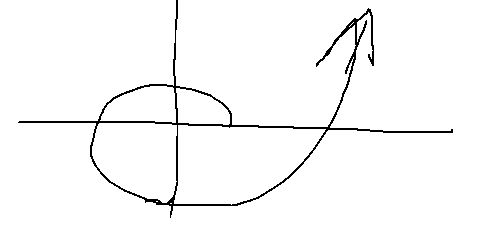
\includegraphics[width=.4\linewidth]{lec6/10_mikh_example4a}

При $ n = 7 $ система на картинке неустойчива ( $ \Delta \phi = \frac{5}{2} \pi \overset{\eqref{eq:mikhailov}}\Rightarrow m = 1 $, один неустойчивый корень).

\textbf{Иной пример.}

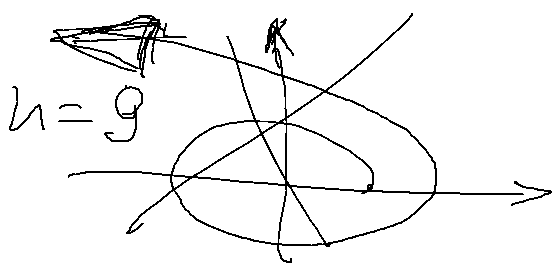
\includegraphics[width=.4\linewidth]{lec6/11_mikh_example4b}

При $ n = 9 $ такой годограф невозможен.
Такой системы просто не может быть, ни устойчивой, ни неустойчивой.

\textbf{Вывод:} приращение аргумента зависит от чётности порядка системы.
Если порядок системы нечётный, годограф должен заканчиваться в нечётном квадранте (вне зависимости от того, устойчива ли система). \\

\textbf{Более конструктивный пример:} инерционное звено

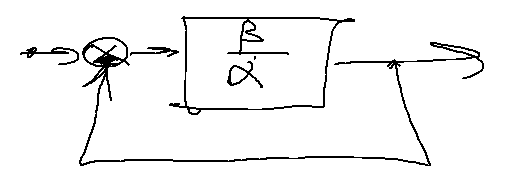
\includegraphics[width=.4\linewidth]{lec6/16_mikh_bound_scheme}

\begin{align*}
	&  H(p) = \frac{1}{Tp + 1} \\
	& \alpha(p) = Tp + 1 \\
	& \alpha(j \omega) = 1 + j \omega T \\
\end{align*}

Кривая здесь -- просто прямая:

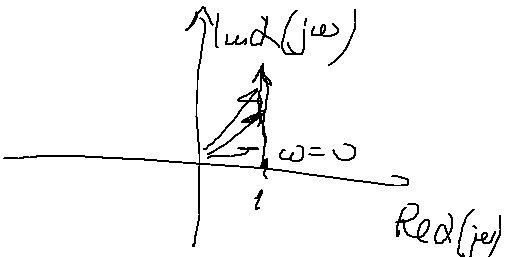
\includegraphics[width=.4\linewidth]{lec6/12_mikh_example5a}

$$ \begin{cases}
    \Delta \phi = \frac{\pi}{2} \\
    n = 1
\end{cases} \overset{\eqref{eq:mikhailov}}\Rightarrow m = 0, \text{система устойчива} $$

Если же  $ H(p) = \frac{1}{Tp - 1} $, рисунок зеркальный относительно вещественной оси.

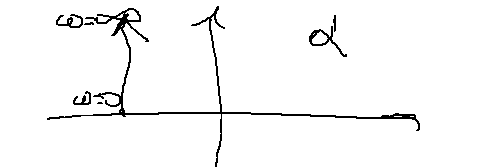
\includegraphics[width=.4\linewidth]{lec6/13_mikh_example5b}

Система при этом становится неустойчивой ($ \Delta \phi = -\frac{\pi}{2} $, один неустойчивый корень).

\subsubsection{Критерий Михайлова. Граница устойчивости}

Граница устойчивости -- ситуация, когда среди корней $ \alpha $ нет положительных, но некоторые находятся на мнимой оси.

Как с помощью критерия Михайлова идентифицировать систему, находящуюся на границе устойчивости?
Необходимое, но не достаточное условие: годограф проходит через ноль.

\textbf{Пример:} $ n=4 $.

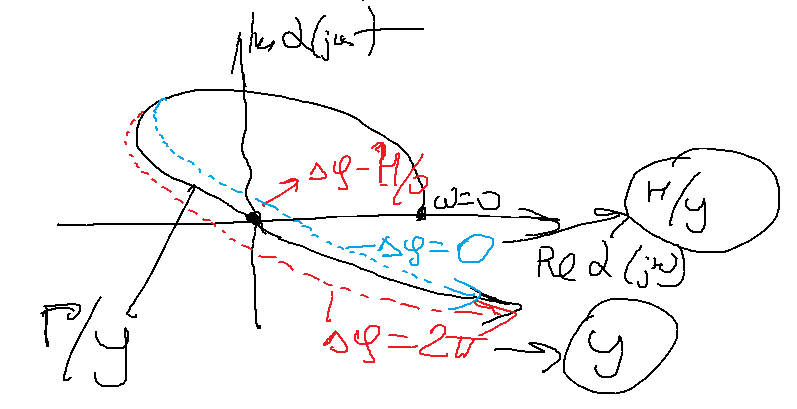
\includegraphics[width=.4\linewidth]{lec6/15_mikh_bound_godograph}

Пошевелим немного годограф в одну сторону (красная кривая) $ \Rightarrow $ система становится устойчивой ($ \Delta \phi = 2 \pi $).
Пошевелим в другую $ \Rightarrow  \Delta \phi = 0$, система неустойчива.

Смотрите-ка, мы на границе устойчивости!

Если бы порядок был $ n = 6 $ (а не $4$), то при смещении в одном случае (синяя кривая) было бы 3 неустойчивых корня с $Re \lambda > 0$; при смещении в другую сторону (красная кривая) был бы 1 неустойчивый корень:

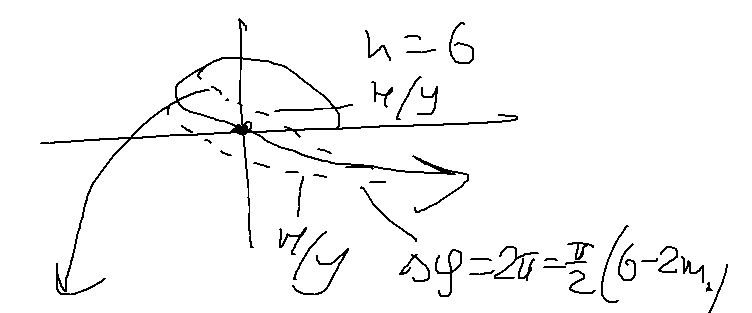
\includegraphics[width=.4\linewidth]{lec6/15_mikh_bound_godograph2}

Следовательно, при $ n = 6 $ система не находится на границе устойчивости.

Зная годограф и $n$, можно восстановить картину расположения корней:
если годограф подвинуть вниз, то $ \Delta \phi = 2 \pi \overset{\eqref{eq:mikhailov}}\Rightarrow m_1 = 1  $; если вверх, то $ \Delta \phi = 0 \overset{\eqref{eq:mikhailov}}\Rightarrow m_2 = 3  $.

Т. о. два корня находятся на мнимой оси и при движении смещаются вправо / влево, один корень справа от мнимой оси (неустойчивый, отмечен красным) и три слева (возможно, комплексные).

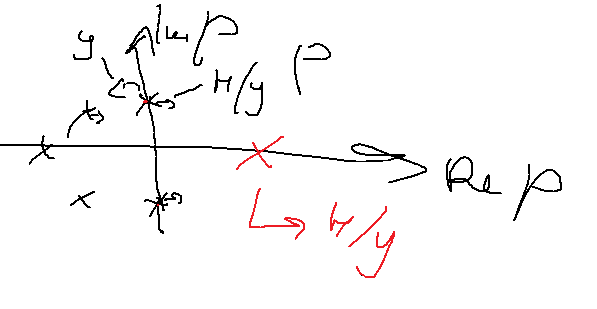
\includegraphics[width=.4\linewidth]{lec6/14_mikh_bound}

\subsubsection{Примеры. Критерий Михайлова для передаточной функции замкнутой цепи}

\textbf{Пример 1.} Пусть
$$ H_{\text{разомкн}} = \frac{K}{p(Tp + 1)} $$
и система с отрицательной единичной обратной связью:

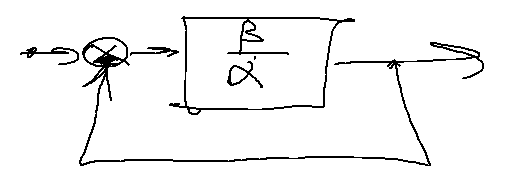
\includegraphics[width=.4\linewidth]{lec6/16_mikh_bound_scheme}

Тогда
$$ H_{\text{замкн}} = \frac{\frac{\beta}{\alpha}}{1 + \frac{\beta}{\alpha}} = \frac{\beta}{\alpha + \beta} = \frac{\beta}{\alpha_{\text{з}}} $$
Отсюда (в общем случае, вне зависимости от вида $ H_{\text{разомкн}} $):
$$ \boxed{ \alpha_{\text{з}} = \alpha + \beta } $$

Проверяем устойчивость по критерию Михайлова:
\begin{enumerate}[noitemsep]
    \item $ \alpha_{\text{з}}(p) = Tp^2 + p + K $
    \item $ \alpha_{\text{з}}(j \omega) = K - T \omega^2 + j \omega $
\end{enumerate}

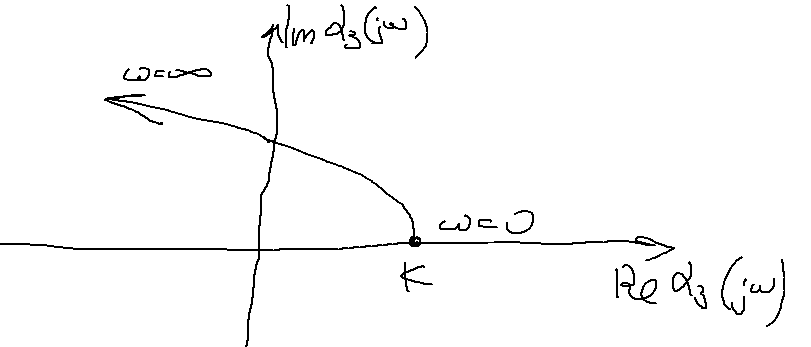
\includegraphics[width=.4\linewidth]{lec6/17_mikh_bound_godograph3}

$$ \Delta \phi = \pi \Rightarrow \text{ система устойчива } $$

\textbf{Пример 2.} Требуется найти $ K_{\text{крит}} $ (критическое значение константы, при котором система на границе устойчивости) для системы третьего порядка:
$$ H_{\text{разомкн}} = \frac{K}{p(T_1 p + 1)(T_2 p + 1)} $$

где константы $ T_1, T_2 > 0 $.

Решение:

\begin{align*}
	& \alpha = T_1 T_2 p^3 + (T_1 + T_2) p^2 + p + K \text{ (необх. условие Стодола выполнено)} \\
    & \alpha(j \omega) = K - (T_1 + T_2) \omega^2 + j \omega (1 - T_1 T_2 \omega^2) \\
\end{align*}

Рисуем годограф: стартуем из точки на вещественной оси; в пределе при $ \omega \to \infty $ находимся в третьем квадранте, причём вещественная часть будет больше мнимой.

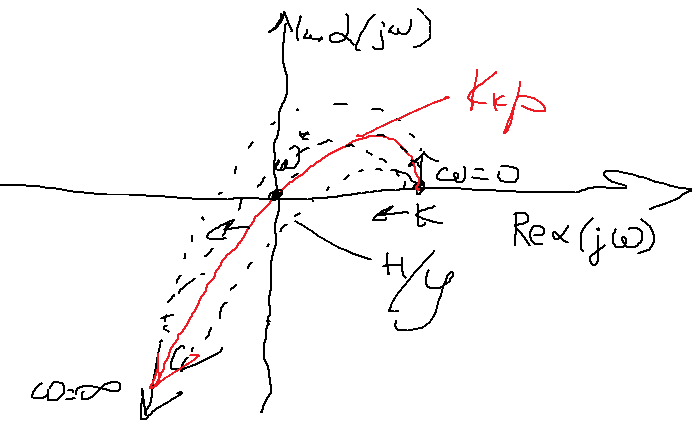
\includegraphics[width=.4\linewidth]{lec6/18_mikh_bound_godograph4}

Ищем критическое значение константы.

\begin{align*}
    & K_{\text{крит}} : \exists \omega^* : \alpha(j \omega^*) = 0 \\
    & j \omega^* (1 - T_1 T_2 \omega^{*2}) = 0 \Rightarrow \omega^* = \frac{1}{\sqrt{T_1 T_2}} \\
    & K - (T_1 + T_2) \omega^{*2} = 0 \Rightarrow K_{\text{крит}} = \frac{T_1 + T_2}{T_1 T_2} \\
\end{align*}

Система устойчива, если $ K < K_{\text{крит}} $.

Естественно, такой же вывод можно сделать по критерию Гурвица -- произведение средних коэффициентов должно быть в устойчивой системе больше произведения крайних:
$$ T_1 + T_2 > T_1 T_2 $$

\subsection{Критерий Найквиста}
Найквист (1932) -- американец.
Чуть посложнее.

Сравнение: Михайлов работает со знаменателем замкнутой цепи $ \alpha_{\text{з}}(j \omega) $, Найквиста -- с дробью разомкнутой $ H_{\text{разомкн}} = \frac{\beta(j \omega)}{\alpha(j \omega)} = \prod H_i $.
По сложности в среднем примерно одно и то же.

Сейчас получим :
$$ \Psi(p) = 1 + H_{\text{разомкн}} = 1 + \frac{\beta}{\alpha} = \frac{\alpha + \beta}{\alpha} = \frac{\alpha_{\text{з}}}{\alpha} $$
Порядок знаменателя $n$, числителя -- $ m \le n \Rightarrow $ порядок $  $ % TODO
$$ \Delta \arg \Psi() $$ % TODO

здесь $ l $ -- количество строго неустойчивых корней знаменателя $ H_{\text{разомкн}} $.

Cтроим годограф $ H_{\text{разомкн}} $ в осях $ Re( \Psi(j \omega) ), Im( \Psi(j \omega)) $

Т. о. для устойчивой системы необходимо и достаточно, чтобы годограф $ H_{\text{разомкн}} $ сделал $ \frac{l}{2} $ оборотов вокруг точки $ (-1;0) $ (это оси $ \Psi $)

Примеры.
% TODO img, img
Число неустойчивых корней знаменателя $ l = 0 $, годограф делает ноль оборотов вокруг точки $ (-1;0) $ (на обеих картинках), и

\subsubsection{Геометрическое правило Цыпкина}
Будем считать число пересечений с лучом $ ( - \infty; -1 ]) $ на вещественной оси: если пересекаем из второго квадранта в третий, добавляем +1; из третьего во второй -- -1; если стартуем из точки на отрицательной вещественной полуоси, добавляем + или $ - \frac{1}{2} $ в зависимости от того, в какую сторону стартуем.
% TODO img

Пример.
$$ H_{\text{раз}} = \frac{2}{p-1}, \thickspace l = 1 $$
$$ H_{\text{раз}}(j \omega) = \frac{2}{j \omega - 1} = \frac{-2 - 2 j \omega}{\omega^2 + 1} $$
% TODO img
% TODO вывод из примера, проверка

\subsubsection{Критические случаи}
У критерия Михайлова нет особых случаев.
У критерия Найквиста есть.

\begin{itemize}[noitemsep]
    \item $ H_{\text{раз}} = \frac{\beta(p)}{p^s \alpha(p)} $ -- плохо, т. к.
    Тогда принцип аргумента применить нельзя, $ \Delta \arg (1 + H_{\text{раз}}(j \omega)) |_0^{\infty} $ -- величина не определённая.

    Как быть? % TODO запутался, не уверен в следующей строке.
    %	Если на мнимой оси $ l $ корней у $ \alpha_{\text{разомкн}} $, $ \Delta \arg \alpha(j \omega) |_{- \infty}^\infty = \pi (n - 2 l) $
    % TODO
    Обходим неприятную точку $ (0;0) $ справа (слева нам неудобно): % TODO
    Модификация принципа аргумента для знаменателя: $\Delta \arg \alpha(p) |_{\text{trajectory}}$

    $$ trajectory = \begin{cases}
        j \omega, \omega < - \varepsilon or \omega > \varepsilon \\
        \varepsilon e^{- j \frac{\pi \omega}{ 2 \varepsilon}}, \omega \in [- \varepsilon; \varepsilon]
    \end{cases} $$
    % TODO
    $$ \Delta \arg [1 + H_{\text{раз}}(p)] |_{traject} =  $$

    $$ H_{\text{раз}}(p) = \begin{cases}
        H_{\text{раз}}(j \omega), \omega > \varepsilon \\
        H_{\text{раз}}(p), p = % TODO a bit
    \end{cases} $$
    $$ H_{\text{раз}}(p) |_{traj, \varepsilon \to 0} = \begin{cases}
        content...
    \end{cases} $$

    Т. о. надо дополнить годограф дугой бесконечно большого радиуса с фазой $ - \frac{\pi}{2}s $ ($ s $ -- кратность нуля как корня знаменателя), которая должна начинаться на положительной полуоси.
    Найдя эту траекторию, считаем число пересечений:

    Итак, разрыв в нуле % TODO

    Для применения правила Цыпкина достаточно брать не бесконечно большую дугу, а любую с радиусом $ > 1 $.

    Пример: интегратор.
    $$ H_{\text{раз}} = \frac{1}{p} $$
    Годограф интегратора, напомним, таков:
    % TODO img

    $ s = 1, l = 0 $.
    Дополняем эту траекторию дугой.
    % TODO

    Ещё один пример:
    $$  $$

    Проверка: $ \alpha_{\text{з}} = p^{} $ % TODO
    \item Второй критический случай: комплексно сопряжённые
    $$ H_{\text{раз}}(p) = \frac{\beta(p)}{\prod(p^2 + \omega_\mu^2) \alpha(p)} $$
    % TODO img
    <<Прыжок>> на $\pi$ или $-\pi$, разрыв

    Выход: обходим корень по дуге бесконечно малого радиуса.
    Тогда изменение аргумента вспомогательной функции от $p$ есть % TODO

    Итак, если у нас второй критический случай (в знаменателе есть чисто мнимые корни), то дополняем годограф дугой бесконечно большого радиуса с радиусом $ - \pi \cdot \text{кратность корня} $, после чего уже можно пользоваться правилом Цыпкина.

    Пример.
    \begin{align*}
        & H_{\text{раз}}(p) = \frac{p}{p^2 + 1}, \thickspace l = 0  \\
        % TODO
    \end{align*}

    То же самое, но со знаком минус:
    \begin{align*}
        & H_{\text{раз}}(p) = \frac{-p}{p^2 + 1}, \thickspace l = 0  \\
        % TODO
    \end{align*}
\end{itemize}

\subsubsection{Границы устойчивости в критерии Найквиста}

Если в критерии Михайлова точка, подозрительная на границу устойчивости -- $ (0;0) $, то здесь -- $ (-1;0) $.
Как исследовать?
Точно так же: пошевелить.

Пример:
% TODO
\begin{align*}
    & \phi = 0 - \left[\frac{num}{den}\right] \\
    & \\ % TODO
    & K_{\text{крит}} = \frac{T_1 + T_2}{T_1 T_2} \text{ (совпадает с результатом, полученным по критерию )} \\
\end{align*}

\begin{itemize}[noitemsep]
    \item
    \item
\end{itemize}

\end{document}
